%%%%%%%%%%%%%%%%%%%%%%%%%%%%%%%%%%%%%%%%%
% Masters/Doctoral Thesis 
% LaTeX Template
% Version 2.5 (27/8/17)
%
% This template was downloaded from:
% http://www.LaTeXTemplates.com
%
% Version 2.x major modifications by:
% Vel (vel@latextemplates.com)
%
% This template is based on a template by:
% Steve Gunn (http://users.ecs.soton.ac.uk/srg/softwaretools/document/templates/)
% Sunil Patel (http://www.sunilpatel.co.uk/thesis-template/)
%
% Template license:
% CC BY-NC-SA 3.0 (http://creativecommons.org/licenses/by-nc-sa/3.0/)
%
%%%%%%%%%%%%%%%%%%%%%%%%%%%%%%%%%%%%%%%%%

%----------------------------------------------------------------------------------------
%	PACKAGES AND OTHER DOCUMENT CONFIGURATIONS
%----------------------------------------------------------------------------------------

\documentclass[
11pt, % The default document font size, options: 10pt, 11pt, 12pt
%oneside, % Two side (alternating margins) for binding by default, uncomment to switch to one side
english, % ngerman for German
singlespacing, % Single line spacing, alternatives: onehalfspacing or doublespacing
%draft, % Uncomment to enable draft mode (no pictures, no links, overfull hboxes indicated)
%nolistspacing, % If the document is onehalfspacing or doublespacing, uncomment this to set spacing in lists to single
%liststotoc, % Uncomment to add the list of figures/tables/etc to the table of contents
%toctotoc, % Uncomment to add the main table of contents to the table of contents
%parskip, % Uncomment to add space between paragraphs
%nohyperref, % Uncomment to not load the hyperref package
headsepline, % Uncomment to get a line under the header
%chapterinoneline, % Uncomment to place the chapter title next to the number on one line
%consistentlayout, % Uncomment to change the layout of the declaration, abstract and acknowledgements pages to match the default layout
]{MastersDoctoralThesis} % The class file specifying the document structure

\usepackage[utf8]{inputenc} % Required for inputting international characters
\usepackage[T1]{fontenc} % Output font encoding for international characters

\usepackage{mathpazo} % Use the Palatino font by default

\usepackage[backend=bibtex,style=authoryear,natbib=true]{biblatex} % Use the bibtex backend with the authoryear citation style (which resembles APA)

\addbibresource{example.bib} % The filename of the bibliography

\usepackage[autostyle=true]{csquotes} % Required to generate language-dependent quotes in the bibliography

%----------------------------------------------------------------------------------------
%	MARGIN SETTINGS
%----------------------------------------------------------------------------------------

\geometry{
	paper=a4paper, % Change to letterpaper for US letter
	inner=2.5cm, % Inner margin
	outer=3.8cm, % Outer margin
	bindingoffset=.5cm, % Binding offset
	top=1.5cm, % Top margin
	bottom=1.5cm, % Bottom margin
	%showframe, % Uncomment to show how the type block is set on the page
}

%----------------------------------------------------------------------------------------
%	THESIS INFORMATION
%----------------------------------------------------------------------------------------

\thesistitle{Automated deployment and performance analysis of a white-label web application} % Your thesis title, this is used in the title and abstract, print it elsewhere with \ttitle
\supervisor{Thomas \textsc{Clauwaert}} % Your supervisor's name, this is used in the title page, print it elsewhere with \supname
\examiner{} % Your examiner's name, this is not currently used anywhere in the template, print it elsewhere with \examname
\degree{Bachelor of applied computer science} % Your degree name, this is used in the title page and abstract, print it elsewhere with \degreename
\author{Niek \textsc{Candaele}} % Your name, this is used in the title page and abstract, print it elsewhere with \authorname
\addresses{} % Your address, this is not currently used anywhere in the template, print it elsewhere with \addressname

\keywords{} % Keywords for your thesis, this is not currently used anywhere in the template, print it elsewhere with \keywordnames
\university{\href{https://www.howest.be}{Howest}} % Your university's name and URL, this is used in the title page and abstract, print it elsewhere with \univname
\department{\href{http://department.university.com}{Department or School Name}} % Your department's name and URL, this is used in the title page and abstract, print it elsewhere with \deptname
\group{\href{http://researchgroup.university.com}{Research Group Name}} % Your research group's name and URL, this is used in the title page, print it elsewhere with \groupname
\faculty{\href{http://faculty.university.com}{Faculty Name}} % Your faculty's name and URL, this is used in the title page and abstract, print it elsewhere with \facname

\AtBeginDocument{
\hypersetup{pdftitle=\ttitle} % Set the PDF's title to your title
\hypersetup{pdfauthor=\authorname} % Set the PDF's author to your name
\hypersetup{pdfkeywords=\keywordnames} % Set the PDF's keywords to your keywords
}

\begin{document}

\frontmatter % Use roman page numbering style (i, ii, iii, iv...) for the pre-content pages

\pagestyle{plain} % Default to the plain heading style until the thesis style is called for the body content

%----------------------------------------------------------------------------------------
%	TITLE PAGE
%----------------------------------------------------------------------------------------

\begin{titlepage}
	\begin{center}
						
		\vspace*{.06\textheight}
		{\scshape\LARGE \univname\par}\vspace{1.5cm} % University name
		\textsc{\Large Thesis}\\[0.5cm] % Thesis type
						
		\HRule \\[0.4cm] % Horizontal line
		{\huge \bfseries \ttitle\par}\vspace{0.4cm} % Thesis title
		\HRule \\[1.5cm] % Horizontal line
						 
		\begin{minipage}[t]{0.4\textwidth}
			\begin{flushleft} \large
				\emph{Author:}\\
				\href{http://www.johnsmith.com}{\authorname} % Author name - remove the \href bracket to remove the link
			\end{flushleft}
		\end{minipage}
		\begin{minipage}[t]{0.4\textwidth}
			\begin{flushright} \large
				\emph{Supervisor:} \\
				\href{http://www.jamessmith.com}{\supname} % Supervisor name - remove the \href bracket to remove the link  
			\end{flushright}
		\end{minipage}\\[3cm]
						 
						
						 
		\vfill
						
		{\large \today}\\[4cm] % Date
		%\includegraphics{Logo} % University/department logo - uncomment to place it
						 
		\vfill
	\end{center}
\end{titlepage}


%----------------------------------------------------------------------------------------
%	QUOTATION PAGE
%----------------------------------------------------------------------------------------

\vspace*{0.2\textheight}

\noindent\enquote{\itshape Funny or thought provoking quote goes here}\bigbreak

\hfill Someone, somewhere

%----------------------------------------------------------------------------------------
%	ABSTRACT PAGE
%----------------------------------------------------------------------------------------

\begin{abstract}
	\addchaptertocentry{\abstractname} % Add the abstract to the table of contents
	A case study and practical implementation of a white-labeled web application. Starting with an existing application, proceeding with analysis of the current implementation and problems, investigating potential solutions and finally implementing them
\end{abstract}

%----------------------------------------------------------------------------------------
%	ACKNOWLEDGEMENTS
%----------------------------------------------------------------------------------------

\begin{acknowledgements}
	\addchaptertocentry{\acknowledgementname} % Add the acknowledgements to the table of contents
	Thanks to Thomas Clauwaert, Serge Morel, en de rest \ldots :)
\end{acknowledgements}

%----------------------------------------------------------------------------------------
%	LIST OF CONTENTS/FIGURES/TABLES PAGES
%----------------------------------------------------------------------------------------

\tableofcontents % Prints the main table of contents

\listoffigures % Prints the list of figures

\listoftables % Prints the list of tables

%----------------------------------------------------------------------------------------
%	ABBREVIATIONS
%----------------------------------------------------------------------------------------

\begin{abbreviations}{ll} % Include a list of abbreviations (a table of two columns)
			
	\textbf{AWS} & \textbf{A}mazon \textbf{W}eb \textbf{S}ervices\\
	\textbf{CMS} & \textbf{C}ontent \textbf{M}anagement \textbf{S}ystem\\
	\textbf{IaC} & \textbf{I}nfrastructure \textbf{a}s \textbf{C}ode\\
			
\end{abbreviations}


%----------------------------------------------------------------------------------------
%	DEDICATION
%----------------------------------------------------------------------------------------

\dedicatory{For/Dedicated to/To my\ldots} 

%----------------------------------------------------------------------------------------
%	THESIS CONTENT - CHAPTERS
%----------------------------------------------------------------------------------------

\mainmatter % Begin numeric (1,2,3...) page numbering

\pagestyle{thesis} % Return the page headers back to the "thesis" style

% Include the chapters of the thesis as separate files from the Chapters folder
% Uncomment the lines as you write the chapters

\chapter{Intro} % Main chapter title

\label{Chapter1} % For referencing the chapter elsewhere, use \ref{Chapter1} 

%----------------------------------------------------------------------------------------

% Define some commands to keep the formatting separated from the content 
\newcommand{\keyword}[1]{\textbf{#1}}
\newcommand{\tabhead}[1]{\textbf{#1}}
\newcommand{\code}[1]{\texttt{#1}}
\newcommand{\file}[1]{\texttt{\bfseries#1}}
\newcommand{\option}[1]{\texttt{\itshape#1}}

%----------------------------------------------------------------------------------------

\section{How it used to be}

Stampix is a startup that prints free photos for clients. Every client gets their own branded web application.

This involves:

\begin{itemize}
	\item Storing all brand-related content in a CMS (Contentful)
	\item Pulling in all that content during app runtime
	\item Deployments for new clients require a lot of manual configuration / dev work
	\item There's no automated tests, which can cause broken deployments if not careful
\end{itemize}

This had a few problems which I will explain in detail later \ldots

%----------------------------------------------------------------------------------------

\section{Solutions}

Following are the methods used to improve this workflow. Each method will probably get it's own detailed chapter later?

\begin{itemize}
	\item Using a static site generator to build web app and assets during build time
	\item Automated testing
	\item Deploying each built application to AWS
\end{itemize}
% Chapter Template

\chapter{Defining the problem} % Main chapter title

\label{Chapter2} 

%----------------------------------------------------------------------------------------
%	SECTION 1
%----------------------------------------------------------------------------------------

\section{Performance}

One of the main bottlenecks with the current approach is the requests to the CMS. When a user visits the site, they first have to load the basic static files from the server. 
This will only load a skeleton of the application though. Depending on what domain name the user is visiting (companyX.stampix.com or companyY.stampix.com), the application will send requests to the CMS to load appropriate images and texts.

This whole process results in a long time before the user can actually start using the application. This paper aims to create a solution that will make this significantly faster.

To support different assets for different clients, the current implementation loads the assets during runtime. 
If loading assets is moved from runtime to build time with a static site generator, the methodology for deploying the application must support this. 
In effect, this means that requests to the CMS will happen during the build scripts.

The main disadvantage of making this distinction during runtime is that users have to wait for the logic and requests to have ran.
By selecting the required assets during build time, users are instantly served the right assets which boosts performance.

\section{Modularity}

Stampix has many clients and every client has individual needs. One client might want to block any NSFW pictures while another doesn't mind these types of pictures and instead wants different functionality.
This means the web application must remain modular enough to support these different "add-ons". This problem can be solved by writing code that supports this and the exact implementation is outside the scope of this paper. 
However, it is an important point and the solution this paper proposes must support it.


\section{Changes to CI/CD}

Moving the process of loading assets from the CMS to build time rather than run time means some changes will need to happen to the CI/CD process.
Whenever new code is written for the web app, builds must be started for each client. This means, if Stampix has 100 active clients, 100 builds must happen.
In the past, this was only 1 build. These deployments cannot happen serially. If Stampix scales to thousands of active clients, each deploy will take several hours or even days to complete.
Instead, the CI/CD process should work in parallel to create a build for every client. This will ensure speedy deployments (in theory, a deployment will take as much time as one build, regardless of how many builds actually happen).

Furthermore, when changes happen to the assets inside the CMS, it should also start new builds. In practice, this could be implemented with a webhook.

When using a webhook, the CMS will send a message to a web service, controlled by Stampix. This service will validate the message, format it as needed and then forward it to the CI platform which will start the pipeline.

\section{Summing up}

\begin{itemize}
	\item How can we improve the performance of the web application during runtime?
	\item How do we make sure that the solution is flexible enough to support all (or as many as possible) current and future, unknown requirements?
	\item How does the process of deployment (CI/CD) change?
\end{itemize} 
% Chapter Template

\chapter{Theory} % Main chapter title

\label{Chapter3} 

%----------------------------------------------------------------------------------------
%	SECTION 1
%----------------------------------------------------------------------------------------

\section{Static site generators}

Static site generators take your app and build it before serving to users. 
This means users receive plain HTML files. This moves a large computational burden from run time to build time which results in significantly faster load times for users.
Furthermore, this approach allows for more aggressive and efficient caching.

\subsection{Nextjs}

Nextjs\footnote{https://nextjs.org/} is a React framework. Not explicitly a static site generator but has support for it. 
Nextjs has support for a ton of interesting features, 

\begin{itemize}
	\item Image optimization
	\item Hybrid static site generation and server side rendering
	\item Internationalization
	\item Typescript support
\end{itemize}

It is important to note that Nextjs heavily uses server side rendering. If used in the end result, the deployment should support this. 
This can be achieved by using Lambda, Lambda@edge or Cloudfront functions.  

\subsubsection{Serverless server side rendering}

As noted, Nextjs uses server side rendering. 
This improves performance as it allows the server to render a page instead of the client.
Servers can have a lot more computing power than the average consumer workstation or mobile.

This does mean that a lot of round-trips will happen between the client and the server. 
Since performance is a key component of the solution here, the solution should try to minimize this.

Luckily, AWS offers a few solutions for this. 
The simplest solution is to use regular lambda functions. 
This will work fine, however the location where this lambda function runs might be very far away from the client, resulting in a larger than desired network latency.
This can be mitigated by using the Lambda@Edge technology from AWS. Instead of running the lambda function in the main AWS data center, it instead runs in the regional edge location.
Regional edge locations are significantly closer to the user, which helps with latency but it is still far removed.
Going one step further, AWS also offers Cloudfront functions. These are functions that run the closest to the client as currently possible.

\begin{figure}[htb!]
	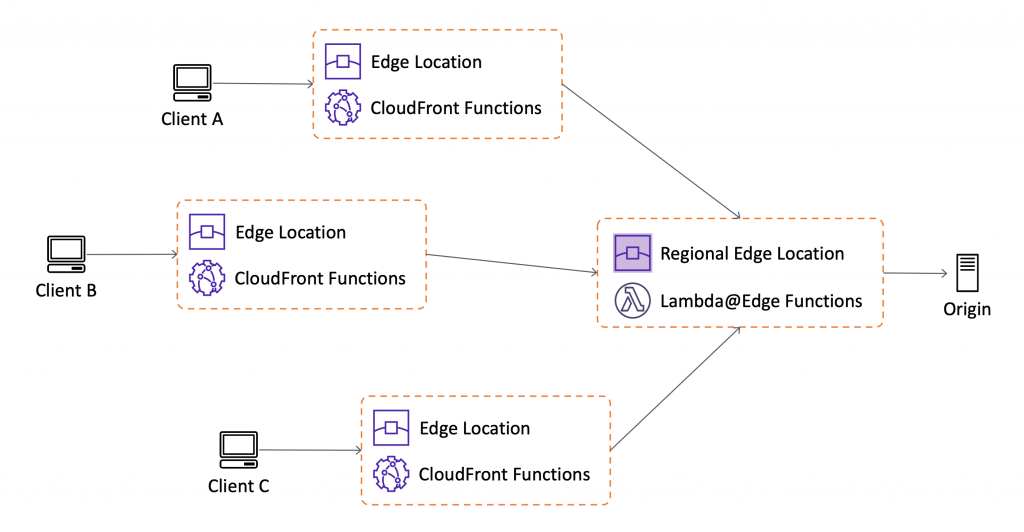
\includegraphics[scale=0.5]{@edge}{}
	\caption{AWS solutions for running code @edge \cite*{aws@edge}}
	\label{fig:@edge}
\end{figure}


\subsection{Gatsby}

Gatsby\footnote{https://www.gatsbyjs.com/} is a static site generator at heart. It is one of the most popular frameworks around \cite{jamstackorg-generators}

\begin{itemize}
	\item Static site generation leads to better performance
	\item Image optimization
	\item Large plugin ecosystem
\end{itemize}



\section{Cypress}

Cypress\footnote{https://www.cypress.io/} is a tool made to run automated end-to-end tests in a browser. 

This research will use Cypress for it's simple API to control browsers programmatically. It will allow us to define the performance benchmarks as code and easily run that on the different PoC applications.

\section{Strapi}

Strapi\footnote{https://strapi.io/} is an open-source CMS. While Stampix uses a different CMS, this research chose Strapi because it is easy to run locally. 
Because the pipeline is running the CMS locally, it is much easier to create a configuration that the pipeline can reuse across different deployments. 


\section{Docker}

Docker\footnote{https://www.docker.com/} is a tool to run and manage containers. All of the components of our benchmarking pipeline will be "Dockerized": the PoC applications, Strapi and even Cypress. 
By using containers for this, pipelines can be created that are platform independent. 
You, the reader, can run the benchmark on your own computer and you will see similar results as presented in this paper. This is explained more thoroughly in chapter \ref{Chapter4}


\section{Methodology}

To make an educated decision on what framework provides the best performance, a benchmarking pipeline will be created. 
Small, proof of concept applications will be created in the above mentioned frameworks which try to replicate real world behavior as close as possible.

Each PoC application must at least be able to load some assets from the CMS and perform an API request to the backend.


\section{Metrics}

Now that it is defined how this performance benchmark will be created and ran, key metrics can be defined.

\subsection{Largest contentful paint}

\begin{quote}
	Largest Contentful Paint (LCP) is an important, user-centric metric for measuring perceived load speed because it marks the point in the page load timeline when the page's main content has likely loaded—a fast LCP helps reassure the user that the page is useful.
	\hfill \cite{webvitalswebsite}
\end{quote}

LCP is an important metric for us. In the original application, this would happen after the request to the CMS. 
That means LCP will be rather late for the average use.
By using static site generators, it can be assured that all of the content shown to users is served from a very fast CDN. 

\subsection{First input delay}

\begin{quote}
	First Input Delay (FID) is an important, user-centric metric for measuring load responsiveness because it quantifies the experience users feel when trying to interact with unresponsive pages—a low FID helps ensure that the page is usable.
	\hfill \cite{webvitalswebsite}
\end{quote}

FID is a very important metric. When a user visits the website, they want to see content and interact with the site as quick as possible. 
When a site has a large FID, it means users have to waste precious time waiting for the site to fully load. In the performance benchmark, this is measured by total blocking time. 

\subsection{Bundle size}

When a user visits the site, one of the main reasons they have to wait for a site to load is network connectivity. 
If a user has a faster network connection, they can download the static files of the website faster.
This is a part of the system where Stampix has very little control, it is impossible to give the users a better network connection. 
However, what can be done, is make sure that the user has to download the smallest amount of data as possible. 
To achieve this, a technique called minification can be used to take our front end code and make it smaller.

Code written by developers might look something like:

\begin{verbatim}
    function doSomething(parameterName) {
        const aVariableWithALongName = 'foo'
        return aVariableWithALongName + parameterName + 'bar'
    }
\end{verbatim}

After minification, the code will look something like:

\begin{verbatim}
    function a(o){return"foo"+o+"bar"}
\end{verbatim}

Over the entire codebase, shortening the code like this will result in a significantly smaller download size for the user.

%\chapter{Performance analysis}

\label{Chapter4} 

\section{Creating the benchmark}

\subsection{Lighthouse}

In order to measure the performance of a web site, several techniques exist. One of those is a Lighthouse report. 
This report encompasses lots of different metrics which each tell you more about a website. 
Not all of these metrics are performance metrics, some are an indicator for accessibility, others for search engine optimization or other miscellaneous metrics.
Which metrics we will analyse was expanded upon in the previous chapter but I wanted to reiterate why I chose Lighthouse.

Lighthouse is an open source solution which can be ran locally. 
A lot of alternatives to Lighthouse are proprietary, hosted solutions. 
This makes it a lot harder to benchmark the PoCs because they should all get deployed and be accessible from the internet. 
During development of this benchmark, it helped a lot to be able to instantly run a new benchmark with the new code without having to go through a full deployment.

A negative about Lighthouse is that is difficult to run on browsers other than Google Chrome. While it is technically possible to do so, I did not implement this and opted to use a single browser for testing.

\subsection{Docker}

Docker was used to run the benchmark. Every PoC application has a Dockerfile which details the steps of the build. 
Why use Docker when you could also just run the applications directly on the host?
Because using Docker to create images of the applications makes for a reproducible build and allows me to control every parameter of the process.
In theory, it does not matter whether the images are built on Linux or Windows. 
It does not matter which version of node is locally installed, because the version is specified in the Dockerfile.

Furthermore, Docker not only provides more control over the build, it also gives more control and configurability to the runtime. 
By using Docker Compose, I can dictate how containers can talk to each other.

All of this together makes for a more stable and deterministic build process. 
It allows other people, on different machines, to run the same benchmark easily and observe similar results.

It should be noted that the Dockerfiles for each PoC has some slight differences.
While the PoCs are all websites, running them in Docker is not the same. 
In effect, for the Next PoC, the built-in next web server was used while for the Gatsby PoC, an intermediate container running Nginx was used.

\subsection{Jupyter notebook}

The results of this benchmark are lots of numbers. 
Especially when the benchmark is run several times, it quickly becomes infeasible to manually calculate and create graphs.
I solved this by creating a Jupyter notebook which handles all the calculations and graphing. 
The notebook requires a modern version of Python installed. 
Python 3.8.5 was used for the graphs in this paper but as long as you use at least Python 3, it should work fine.

To run the notebook, a few dependencies are required. 
These can be viewed at the top of the notebook and can be installed with the Python package manager, pip. 


\section{Running the benchmark}

In order to see which of the web technologies scores best, a performance benchmark was created. 
This benchmark uses Cypress to run a Lighthouse report for each PoC application.

The steps for running it are as follows:

\begin{enumerate}
	\item Start the CMS containers.
	      \begin{verbatim}
			docker-compose -f docker-compose-deps.yml up -d
	      \end{verbatim}
	      This will start a Postgres database and Strapi, the CMS. 
	      These must be ran before the others since the build scripts for the web applications require Strapi.
	      The git repo for this paper includes bootstrapped data for Strapi, with a campaign already configured, complete with starting data.
	\item Build all the PoC applications
	      	      	      	      	      	      	      	      	      	      	      	      	      	      	      	      	      	      	      	      	      	      	      	      	      	      	      	      	      	      	      	      	      	      	      	      	      	      	      	      	
	      \begin{verbatim}
			docker-compose -f docker-compose-bench.yml up -d
	      \end{verbatim}
	      This will build the applications and start the containers. 
	      You can access each application in the browser, starting with port 3000. (http://localhost:3000, http://localhost:3001, \dots)
	      	      	      	      	      	      	      	      	      	      	      	      	      	      	      	      	      	      	      	      	      	      	      	      	      	      	      	      	      	      	      	      	      	      	      	      	      	      	      	      
	\item  
	      	      	      	      	      	      	      	      	      	      	      	      	      	      	      	      	      	      	      	      	      	      	      	      	      	      	      	      	      	      	      	      	      	      	      	      	      	      
	      \begin{verbatim}
			cd packages/benchmark
			npm ci
			npm run cypress:open
	      \end{verbatim}
	      	      	      	      	      	      	      	      	      	      	      	      	      	      	      	      	      	      	      	      	      	      	      	      	      	      	      	      	      	      	      	      	      	      	      	      	      	      
	      This will install Cypress and its dependencies. 
	      After running the final command, Cypress will open and you are able to run the benchmark.
	      Reports with raw data will be saved in the packages/benchmark/reports directory.
\end{enumerate}

These are the steps to run the benchmark once. In order to get a statistically relevant measurement, a script in available that will run the benchmark multiple times.
At the top of the script, you'll find a variable TOTAL\_RUNS which you can adjust and will control how many times the benchmark is ran.
It can be run with

\begin{verbatim}
		cd packages/benchmark
		node runBenchmark.js
\end{verbatim}

Results from these benchmarking runs can be found in the file packages/benchmark/finalReport.json

Finally, you will find a Jupyter notebook that does some number crunching and renders the plots at packages/data-analysis/analysis.ipynb

Results with raw data can be found in appendix \ref{appendix:lighthouse-report}

\section{Largest contentful paint}

\begin{figure}[htb!]
	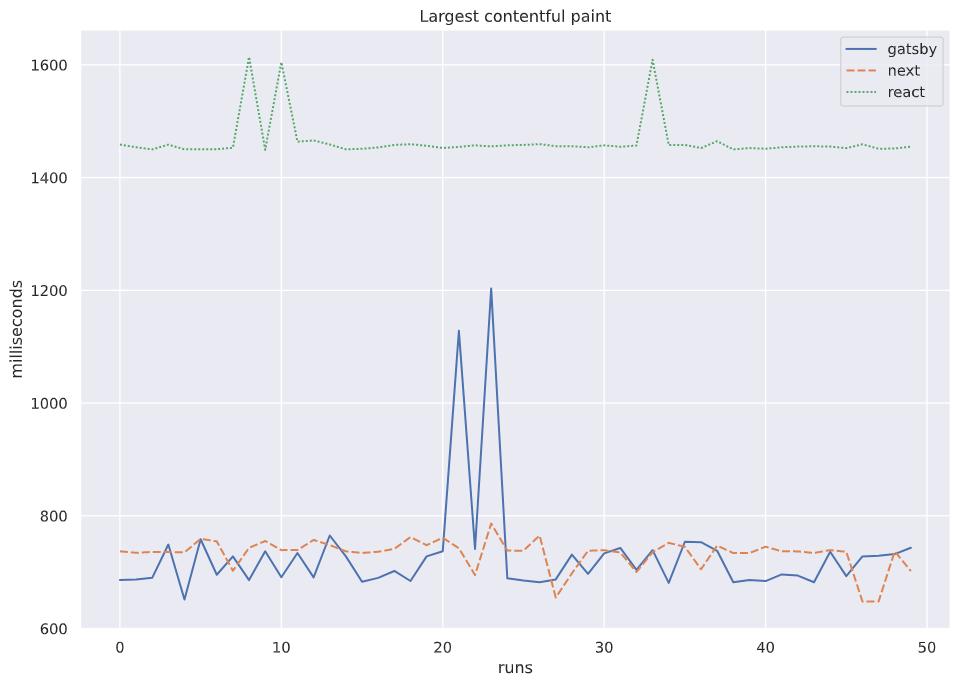
\includegraphics[scale=0.4]{largest_contentful_paint}{}
	\caption{Results of performance benchmark for largest contentful paint}
	\label{fig:largest_contentful_paint}
\end{figure}

In figure \ref{fig:largest_contentful_paint}, it is clear that LCP for a traditional React application is far greater than that of static site generators.

This makes sense: a traditional React application will perform many computational steps during runtime to render the DOM.
Static site generators will perform these computations during the build step.

\section{Total blocking time}


\begin{figure}[htb!]
	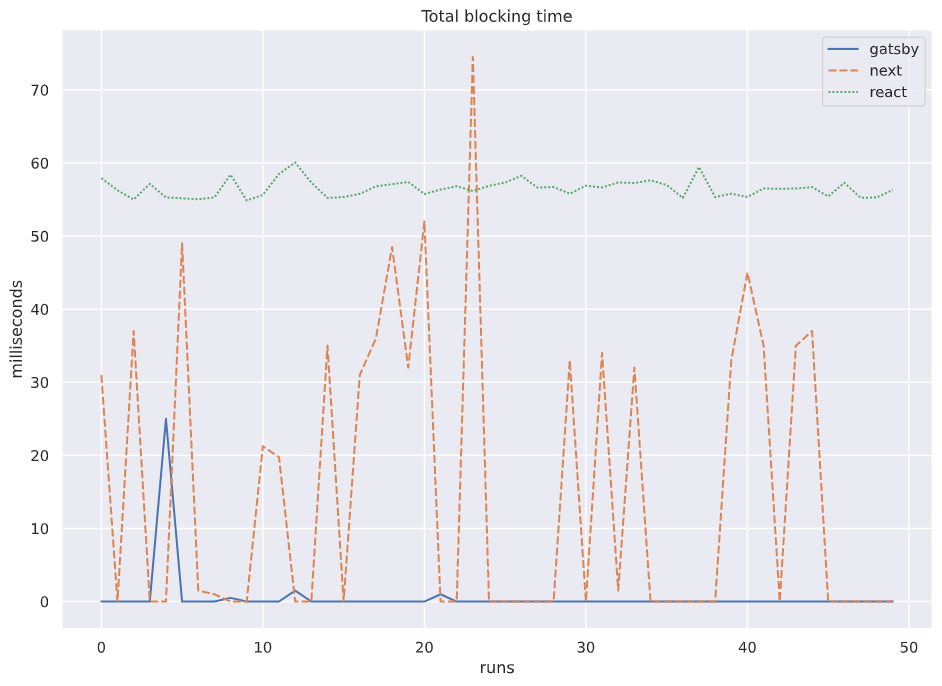
\includegraphics[scale=0.4]{total_blocking_time}
	\caption{Results of performance benchmark for total blocking time}
	\label{fig:total_blocking_time}
\end{figure}

In figure \ref{fig:total_blocking_time}, similar results to the previous figure can be observed
The traditional React application scores much less favorably than the static site generators.
Interestingly, the results for Next seem to spike a lot.


\section{Max potential first input delay}

\begin{figure}[htb!]
	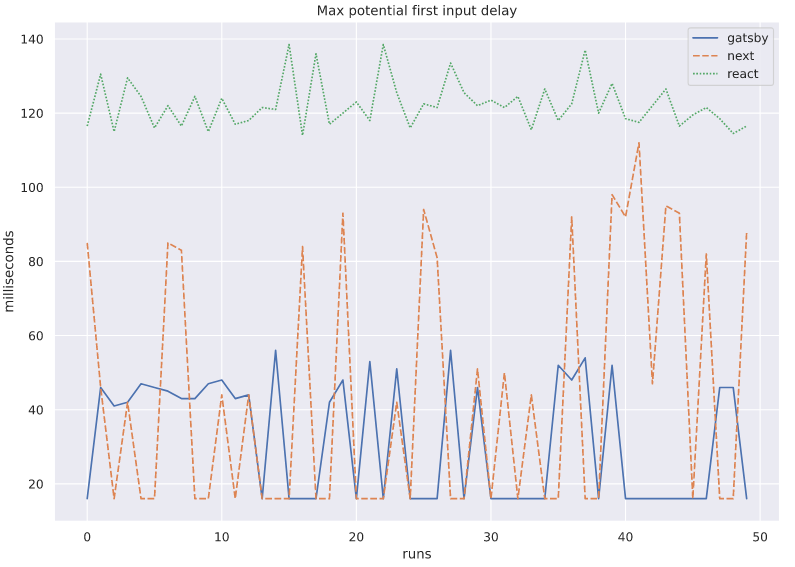
\includegraphics[scale=0.5]{max_potential_first_input_delay}
	\caption{Results of performance benchmark for max potential first input delay}
	\label{fig:max_potential_first_input_delay}
\end{figure}

In figure \ref{fig:max_potential_first_input_delay}, similar results can be observed again. 
The traditional React application scores the worst while the static site generators score significantly better.
It's worth noting that all of the PoCs exhibit irregular measurements, FID fluctuates a lot.
However, on average, the Gatsby PoC scores the best for this metric out of all the PoCs.

\section{Bundle size}

To measure the size of the resulting files after a production build was measured with the Unix command 

\begin{verbatim}
	du -c <directory>
\end{verbatim}

\begin{table}[htb!]
	\begin{center}
		\begin{tabular}{||c c||} 
			\hline
			Site   & Size \\ [0.5ex] 
			\hline\hline
			Gatsby & 3072 \\ 
			\hline
			Next   & 7012 \\
			\hline
			React  & 568  \\[1ex] 
			\hline
		\end{tabular}
		\caption{Total file size of production builds, in kilobytes }
		\label{tbl:bundle_size}
	\end{center}
\end{table}

Looking at table \ref{tbl:bundle_size}, the traditional React application has the smallest bundle here. 
This makes sense, the static generators Next and Gatsby will bundle assets while the traditional React app will fetch these during runtime.

While these results are interesting to see, it should not be a definite factor when deciding which technology to use.
The PoCs created for this paper are very small, a real application would have orders of magnitude more lines of code.
Minification really shines with larger codebases.  
%% Chapter Template

\chapter{Deployment} % Main chapter title

\label{Chapter5} 

\section{Technologies}

There are a lot of IaC solutions out there. Ansible, Terraform, Pulumi, \ldots. 
They all have their own positives and negatives. Choosing the right tool for the job is not easy

Some of the main factors when choosing were

\begin{itemize}
	\item Integration with AWS
	\item Easily scriptable
\end{itemize}

Since Stampix currently runs all their infrastructure on AWS, it makes sense to choose a tool that has good integration with AWS. 
We will be deploying multiple static site builds onto AWS, this means there is some logic involved for each build.
This is why the solution we choose should be easily scriptable: we would rather write the infrastructure as code and not as a declarative language (JSON or YML).




\section{AWS CDK}

\begin{quote}
	The AWS Cloud Development Kit (AWS CDK) is an open source software development framework to define your cloud application resources using familiar programming languages.
	\hfill \cite{awscdk}
\end{quote}

I chose AWS CDK because 

\begin{itemize}
	\item it is made by AWS, so the integration with AWS will be great
	\item it allows us to write infrastructure as javascript code
\end{itemize}

Being able to use Javascript is a big bonus since Javascript is the main language used at Stampix. Everyone in the team knows it well.

\section{Configuration}

As mentioned earlier, every static site needs a separate configuration. 
This configuration will determine what client the build is for, allowing us to fetch the right assets from the CMS. 
Furthermore, this configuration will also allow us to enable or disable certain modules. 

In the proof of concept, this configuration is a static JSON document (see the file packages/infra/config.json). This JSON document does not have to be a static file though. 
It could come from the CMS or even a custom application. 
The goal is to make sure that non-technical people can create deployments. This means that they should not be editing straight JSON files.
Instead, the person creating the deployment should be guided through a form in order to create this configuration. 
To make this experience as smooth as possible, I recommend creating a custom application to create these configs. However, I consider this outside the scope of this paper.


\section{Build and deployment flow}

In order to deploy websites, we need to use a domain name. We will use AWS' managed DNS service, Route 53 \footnote{https://aws.amazon.com/route53/}

The first thing that happens is the configuration JSON is retrieved and read. Based on the contents, several builds of the frontend application are started.

The built files get stored inside S3 \footnote{https://aws.amazon.com/s3/}. Every campaign gets a separate bucket.

The script will also provision TLS certificates via AWS. 
Finally, a CloudFront \footnote{https://aws.amazon.com/cloudfront/} distribution is set up. This will make sure the static files get served when someone visits our sites. 

%----------------------------------------------------------------------------------------
%	THESIS CONTENT - APPENDICES
%----------------------------------------------------------------------------------------

\appendix % Cue to tell LaTeX that the following "chapters" are Appendices

% Include the appendices of the thesis as separate files from the Appendices folder
% Uncomment the lines as you write the Appendices

\chapter{Lighthouse report} % Main appendix title

\label{appendix:lighthouse-report}

This is the output of 50 runs of the benchmarking pipeline.
This output is already truncated to only include the most interesting data.
To see the full data, please see the files in packages/benchmark/reports

\lstinputlisting{Appendices/finalReport.json}

%\include{Appendices/AppendixB}
%\include{Appendices/AppendixC}

%----------------------------------------------------------------------------------------
%	BIBLIOGRAPHY
%----------------------------------------------------------------------------------------

\printbibliography[heading=bibintoc]

%----------------------------------------------------------------------------------------

\end{document}  
